
\documentclass[11pt]{article}


% Use wide margins, but not quite so wide as fullpage.sty
\marginparwidth 0.2in 
\oddsidemargin 0.1in 
\evensidemargin 0.1in 
\marginparsep 0.1in
\topmargin 0.1in 
\textwidth 6.5in \textheight 8 in
% That's about enough definitions

% multirow allows you to combine rows in columns
\usepackage{multirow}
% tabularx allows manual tweaking of column width
\usepackage{tabularx}
% longtable does better format for tables that span pages
\usepackage{longtable}
\usepackage{graphicx}
\usepackage{amssymb} % needed for math
\usepackage{amsmath} % needed for math 
\usepackage{color}
\definecolor{dkgreen}{rgb}{0,0.6,0}
\definecolor{gray}{rgb}{0.5,0.5,0.5}
\definecolor{mauve}{rgb}{0.58,0,0.82}
\usepackage{hyperref}  
\usepackage{listings}

\begin{document}

\author{İbrahim Burak Tanrıkulu, 21827852}
\title{BBM436 Microprocessors Lab.\\Fall 2020\\Assignment 3\\"Hello world" for microprocessor circuits}
\maketitle

\section{Microprocessor circuit design}
Microprocessors have registers to store data, but its not enough. Thus we use RAM and ROM.
\newline 8086 processor has 20-bit address bus and 16-bit data bus. So, we can use 1 MB memory.
\newline In this experiment, i used just 8-bit addresses. Because its too enough to run a "Hello World" program.
\newline Firstly, i connected our RAM and ROM to our 8086 microprocessor with address latch and transceiver.
\begin{figure}[h!]
	\centering
	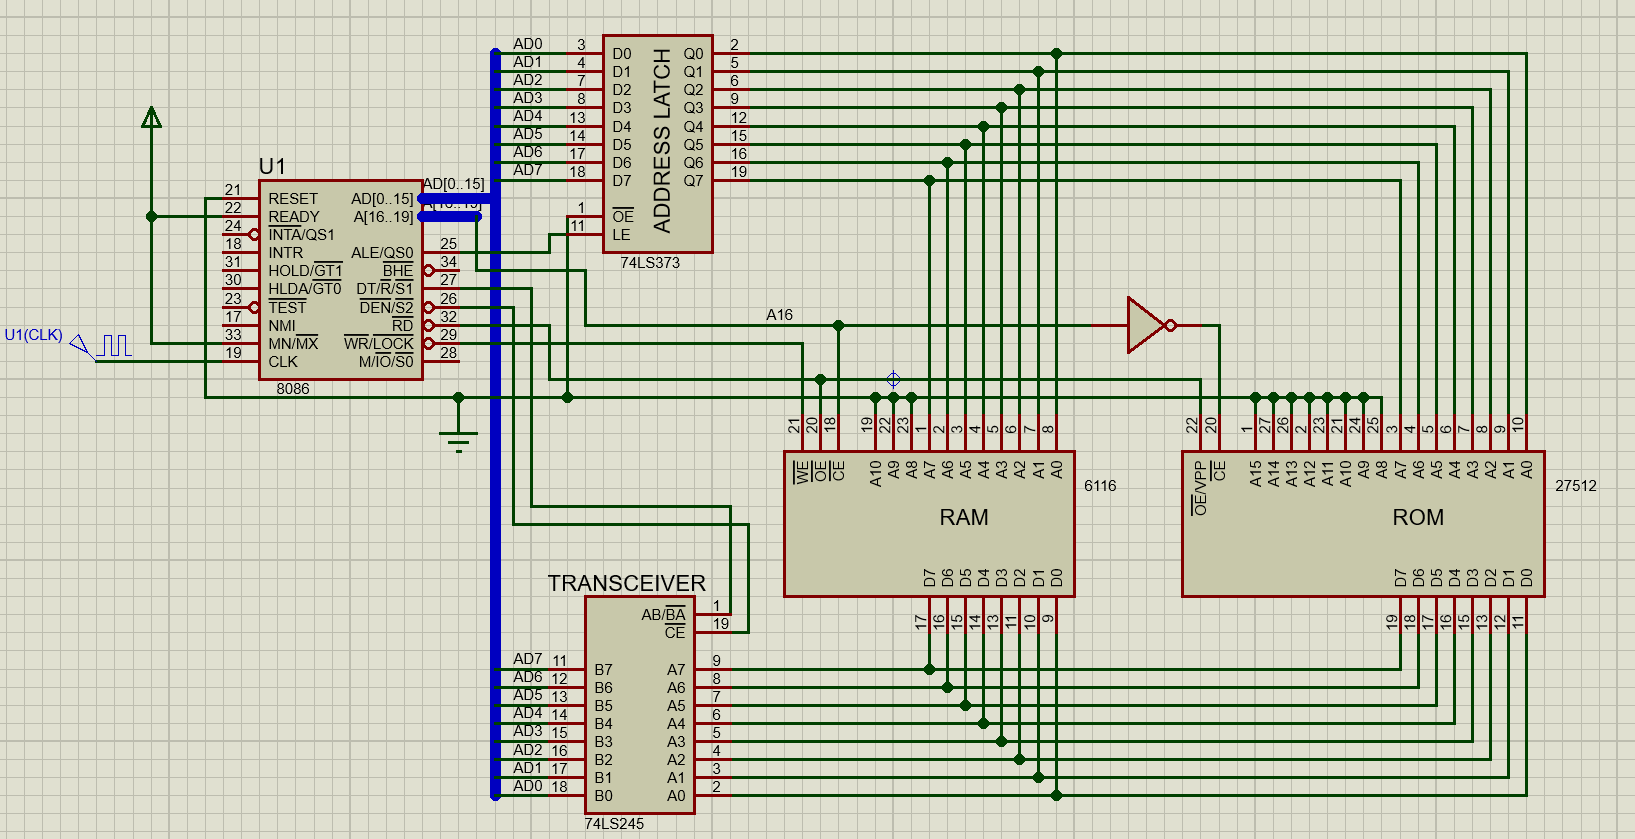
\includegraphics[width=15cm]{Tasarım.png}
	\caption{First microprocessor circuit design}
	\label{fig:Tasarım1}
\end{figure}
\newline
Then, i realized that our program will be in ROM. So we must set Reset Vector to ROM's starting adress. Reset Vector in 8086 is 0xFFFF0 . Thus i redesigned that circuit.
\begin{figure}[h!]
	\centering
	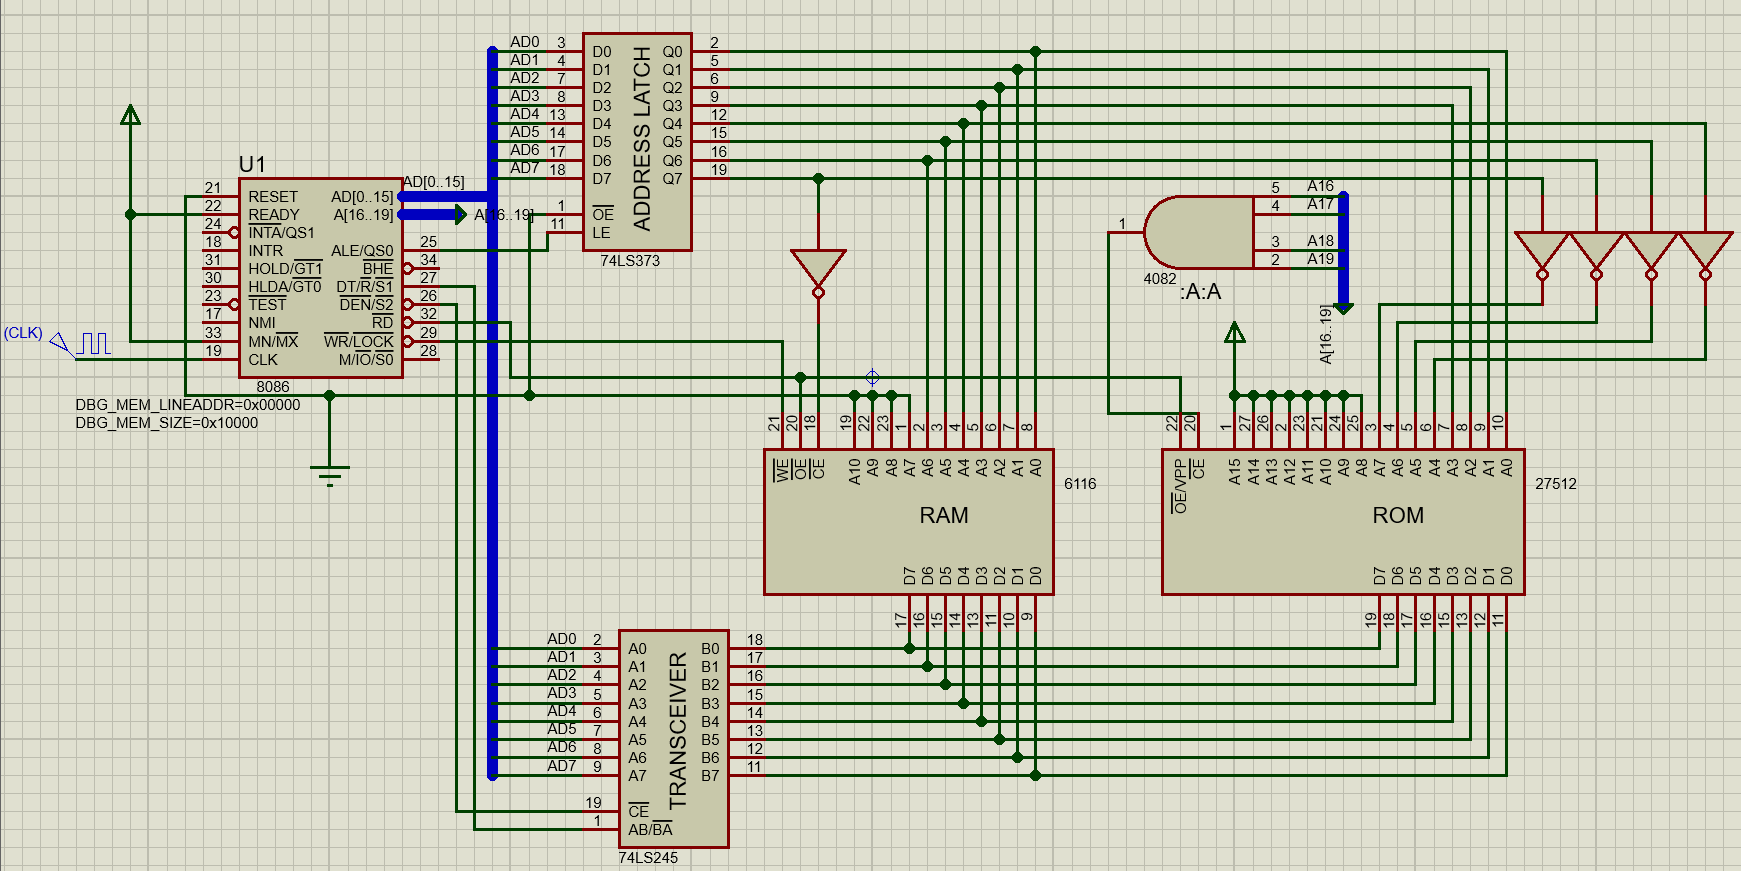
\includegraphics[width=14cm]{Tasarım2.png}
	\label{fig:Tasarım2}
\end{figure}
\section{"Hello World" program}
Our design was completed and now, that was time to test it. I write an assembly code and tested it with this circuit. But it wasn't working. Then i researched internet to solve this problem. But i couldn't found anyting useful. So i decided that i will show that program works correctly in different way. Thus, i used LCD to write "Hello World". 
\newline In proteus, there is "Internal memory" in 8086. So i didn't connect any memory to 8086. Just used address latch and 8255A (Programmable Peripheral Interface" to manage input-outputs. 
\begin{figure}[h!]
        \centering
        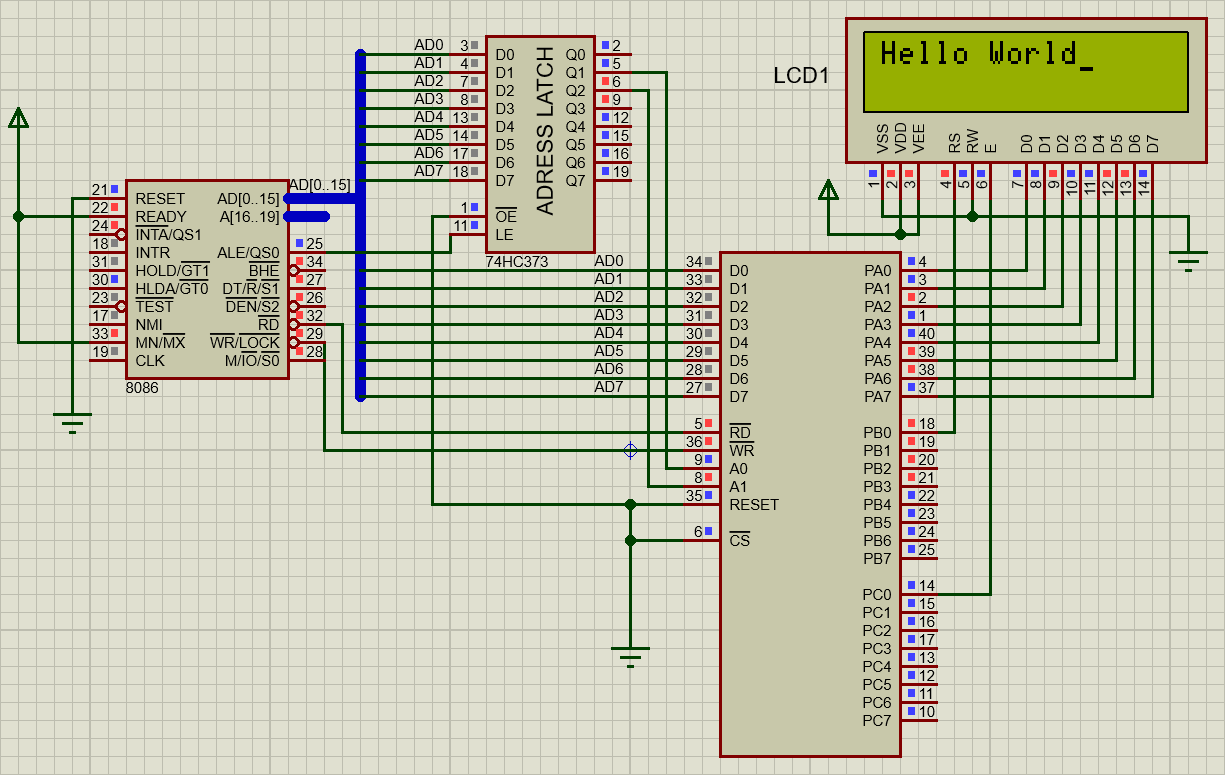
\includegraphics[width=10cm]{LCD.png}
        \label{fig:LCD}
\end{figure}

\end{document}
